\documentclass[brazil]{beamer}
\usepackage[brazil]{babel}
\usepackage[utf8]{inputenc}
\usepackage{graphicx}
\usepackage{ragged2e}
\usepackage{enumitem}
\usetheme{Madrid}

\title[Defesa: Trabalho de Conclusão de Curso] {Desvendando a Criptografia de Curvas Elípticas}
\subtitle{Propriedades, Métodos e Implementação}

\author[\fontsize{8}{10}{Ruas, I.P. de A.; Paiva, C.R.A.D.; Silva, F.M.S}]{\vspace{0.4cm}Isak Paulo de Andrade Ruas \\ \fontsize{8}{10}{\textit{Sob orientação} \\ Me. Celimar Reijane Alves Damasceno Paiva \\ Me. Fernando Marcos Souza Silva}}

\institute[IFNMG]{
	Instituto Federal do Norte de Minas Gerais \\
	Campus Januária \\
	Curso de Licenciatura em Matemática \\
	\vspace{0.4cm}
}
\date{8 de Março de 2024}
\logo{
\includegraphics[height=1cm]{../Imagens/logo_ifnmg.jpg}}

\newtheorem{observation}{Observação}\theoremstyle{definition}
\newtheorem{definicao}{Definição}\theoremstyle{definition}
\newtheorem{continuacao}{}\theoremstyle{definition}
\newtheorem{proposicao}{Proposição}\theoremstyle{proposicao}

\newtheorem{exemplo}{Exemplo}\theoremstyle{definition}
\newcommand{\N}{\mathbb{N}}
\newcommand{\Z}{\mathbb{Z}}
\newcommand{\Q}{\mathbb{Q}}
\newcommand{\R}{\mathbb{R}}
\newcommand{\C}{\mathbb{C}}
\newcommand{\K}{\mathbb{K}}
\newcommand{\F}{\mathbb{F}}
\newcommand{\md}{\text{ mod }}

\begin{document}
\begin{frame}[plain]
	\maketitle
\end{frame}
\begin{frame}{Agenda}
	\tableofcontents
\end{frame}

% Introdução: Motivação, Metodologia e Objetivos
\section{Introdução: Motivação, Metodologia e Objetivos}
\begin{frame}
	\tableofcontents[currentsection]
\end{frame}
\begin{frame}{Introdução: Motivação, Metodologia e Objetivos}
	\justifying
	\begin{itemize}[label={$\bullet$}]
		\item Motivação para estudar a criptografia e sua importância na era digital.
		\item Metodologia adotada: revisão bibliográfica e criação de uma biblioteca Python.
		\item Objetivos do estudo: compreender e aplicar criptografia de curvas elípticas.
	\end{itemize}
\end{frame}

% Panorama Histórico da Criptografia
\section{Panorama Histórico da Criptografia}
\begin{frame}
	\tableofcontents[currentsection]
\end{frame}
\begin{frame}{Panorama Histórico da Criptografia}
	\justifying
	\begin{itemize}[label={$\bullet$}]
		\item O uso da criptografia desde Júlio César até os tempos modernos.
		\item A evolução da criptografia com novas tecnologias e o surgimento do telégrafo.
		\item Papel atual da criptografia na segurança de dados em um contexto digital crescente.
	\end{itemize}
\end{frame}

% Fundamentos e Características da Criptografia
\section{Fundamentos e Características da Criptografia}
\begin{frame}
	\tableofcontents[currentsection]
\end{frame}
\begin{frame}{Fundamentos e Características da Criptografia}
	\justifying
	\begin{itemize}[label={$\bullet$}]
		\item Conceitos de criptografia simétrica e assimétrica.
		\item Importância de chaves seguras e a diferença entre chave pública e privada.
		\item Escolha entre criptografia simétrica e assimétrica com base em necessidades específicas.
	\end{itemize}
\end{frame}
\begin{frame}{Entendendo a criptografia simétrica}
	\begin{figure}[h!] \centering
		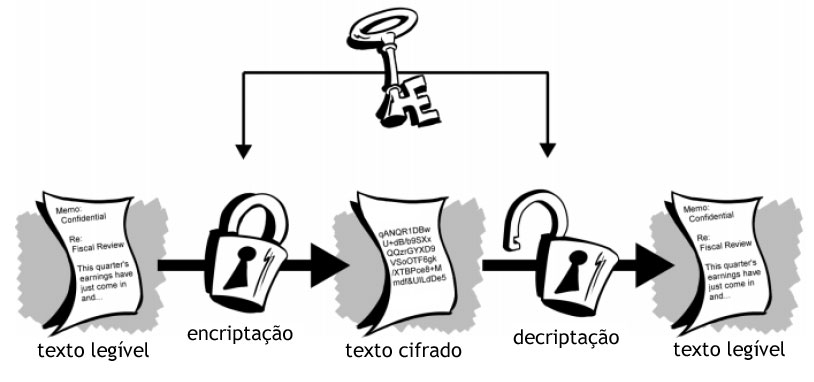
\includegraphics[width=0.7\textwidth]{../Imagens/ilustracao_do_processo_de_criptografia_simetrico}
		\caption{Ilustração do processo de criptografia Simétrico}
		Fonte: Seragiotto, 2023, p. ?
	\end{figure}
\end{frame}
\begin{frame}{Entendendo a criptografia assimétrica}
	\begin{figure}[h!] \centering
		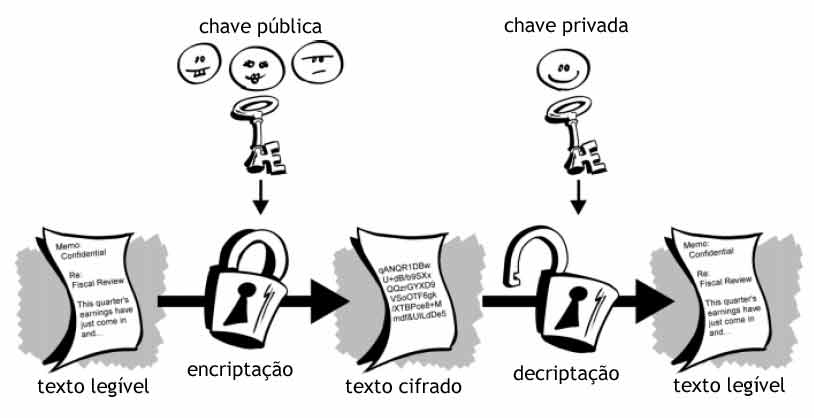
\includegraphics[width=0.7\textwidth]{../Imagens/ilustracao_do_processo_de_criptografia_assimetrico}
		\caption{Ilustração do processo de criptografia Assimétrico}
		Fonte: Seragiotto, 2023, p. ?
	\end{figure}
\end{frame}
% Criptografia com Curvas Elípticas
\section{Criptografia com Curvas Elípticas}
\begin{frame}
	\tableofcontents[currentsection]
\end{frame}
\begin{frame}{Criptografia com Curvas Elípticas}
	\justifying
	\begin{itemize}[label={$\bullet$}]
		\item Definição e propriedades das curvas elípticas em criptografia.
		\item Protocolos de Diffie-Hellman e Massey-Omura para troca de chaves.
		\item Uso do algoritmo de Koblitz para codificar mensagens em curvas elípticas.
		\item Implementação do ECDSA para assinatura digital de mensagens.
	\end{itemize}

\end{frame}

\begin{frame}{Definição de Curvas Elípticas}
	\begin{definicao}
		Uma curva elíptica $E  = \{(x, y) \in \K | (y^2 = x^3 + Ax + B)\}$ no qual $(car(\K) \notin \{2,3\})$
		e ($4A^3 +27B^2 \neq 0)$.
	\end{definicao}

	\begin{definicao}
		$E(\Z_{p}): y^2 \equiv x^3 + Ax + B \pmod{p}$, donde $4A^3 +27B^2 \neq 0 \pmod{p}$
	\end{definicao}


\end{frame}
\begin{frame}{Catálogo de curvas elípticas}

	\begin{figure}[h!] \centering
		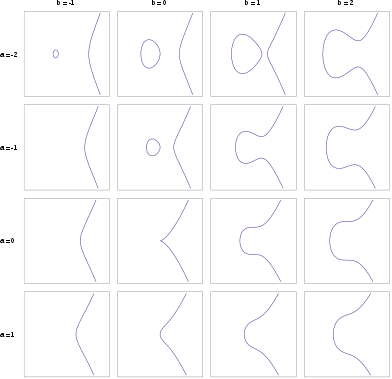
\includegraphics[width=0.5\textwidth]{../Imagens/ellipticcurvecatalog}
		\caption{Catálogo de curvas elípticas}
		Fonte: Domínio Público
	\end{figure}
\end{frame}

\begin{frame}{Protocolo Diffie-Hellman}
 
	\begin{table}[h]\centering
		\vspace*{-0.4cm}
		\caption{Fluxo de passos do protocolo Diffie-Hellman } \label{table:aaf511d5-7922-48dd-b5ad-bf89a728b528}
		\centering
		\begin{tabular}{|p{3cm}|p{3cm}|p{3cm}|}
			\hline
			\textbf{Alice}                                 & \textbf{Canal Público} & \textbf{Bob}                                   \\
			\hline
			Gera aleatoriamente $d_A \in \{1, \ldots, n\}$ &                        & Gera aleatoriamente $d_B \in \{1, \ldots, n\}$ \\
			\hline
			Define $H_A = d_A \cdot G$                     & $H_A \Rightarrow $     & Define $H_B = d_B \cdot G$                     \\
			\hline
			Calcula $S = d_A \cdot H_B$                    & $\Leftarrow H_B$       &                                                \\
			\hline
			&                        & Calcula $S = d_B \cdot H_A$                    \\
			\hline
		\end{tabular}
	 
		\vspace*{0.4cm}Fonte:  Maimon, 2018,  p. 5
	\end{table}
	Em que $n$ é a ordem do gerador da curva $i.e$ $\forall P \in E:  n \cdot P =  \mathcal{O}$.
 

\end{frame}
\begin{frame}{Protocolo Massey-Omura}
	
\begin{table}[h]\centering
	\vspace*{-0.4cm}
	\caption{Fluxo de passos do protocolo Massey-Omura}
	\vspace*{-0.4cm} \label{table:dbb74549-a025-428a-90f4-4efcedbdf9ca}
	\centering
		\begin{tabular}{|p{4cm}|p{3cm}|p{4cm}|}
		 
		\hline
		\textbf{Alice}                                                    & \textbf{Canal Público} & \textbf{Bob}                                                      \\
		\hline
		Representa $m$ como um ponto $M_A \in E$                          &                        &                                                                   \\
		\hline
		Gera aleatoriamente $d_A \in \{1, \ldots, n\}$, $mdc(d_A, n) = 1$ &                        & Gera aleatoriamente $d_B \in \{1, \ldots, n\}$, $mdc(d_B, n) = 1$ \\
		\hline
		Define $H_A = d_A \cdot M_A$                                      & $H_A \Rightarrow $     & Define $H_B = d_B \cdot H_A$                                      \\
		\hline
		$S_A =  (d^{-1}_A  \pmod{n}) \cdot H_B$                           & $\Leftarrow H_B$       &                                                                   \\
		\hline
		& $S_A \Rightarrow $     & $M_A =  (d^{-1}_B \pmod{n}) \cdot S_A $                           \\
		\hline
	\end{tabular}
	\vspace*{0.2cm}\\ % Não apagar esta linha
	Fonte:  Autoria própria.
\end{table}
	\vspace*{-0.2cm}
 Em que $n$ é a ordem do gerador da curva $i.e$ $\forall P \in E:  n \cdot P =  \mathcal{O}$.
\end{frame}

\begin{frame}{Algoritmo de Koblitz }
\begin{definicao}\label{definicao:6c615379-1811-4204-9b1c-fbe2862d9d14}
	$\mathcal{M}$ é a representação de uma mensagem na forma de uma sequência de caracteres, denotada como $\{m_1, m_2, \ldots, m_n\}$, onde $n$ é o tamanho da mensagem. $\mathcal{A} $ é uma sequência numérica, representada como $\{a_1, a_2, \ldots, a_n\}$, que corresponde ao decimal de cada caractere de $\mathcal{M}$ obtido nas tabelas  Unicode ou ASCII. Considerando $b = 2^{16}$ para Unicode e $b = 2^8$ para ASCII, a mensagem cifrada $m$ será obtida por: $m= \sum_{k=1}^{n} a_k \cdot b^{k-1}$ e cada elemento $\{a_1, a_2, \ldots, a_n\}$ poderá ser obtido novamente pela relação a seguir: $a_n = m \div b^{n-1}   \pmod{b}$

	\textit{Nota:  $\div $ neste contexto representa divisão na qual o resultado é o quociente inteiro, sem considerar a parte fracionária. }
\end{definicao}
\end{frame}

\begin{frame}{Algoritmo de Assinatura Digital de Curva Elíptica}

\begin{definicao} \label{definicao:68f23b4d-0cae-44d3-8489-a171e2297efa}
	
	Seja $E(\Z_{p}): y^2 \equiv x^3 + Ax + B \pmod{p}$ curva elíptica, um ponto
	base $G$, um natural $n$, primo, tal que $\forall P \in E: n \cdot P =
	\mathcal{O}$, onde $\mathcal{O}$ é o ponto no infinito, $m$ um numero natural
	representando uma mensagem e $d \in \{1, \ldots, n - 1\}$ representando uma
	chave privada e $Q = d \cdot G$ representando uma chave publica. \justify Para
	$Q$ assinar a mensagem $m$ em $E$, siga os seguintes passos:
 
\end{definicao}
\end{frame}
\begin{frame}{Algoritmo de Assinatura Digital de Curva Elíptica}
	
	\begin{continuacao} \label{definicao:68f23b4d-0cae-44d3-8489-a171e2297efa}
		
	  Para
		$Q$ assinar a mensagem $m$ em $E$, siga os seguintes passos:
		
		1. Escolha um $k \in \N \mid 1 \leq k \leq n - 1 \text{ e } mdc(k, n) = 1$.
		
		2. Calcule $P = k \cdot  G$.
		
		3. Calcule $r = P_x \pmod{n}$. Se $r = 0$ volte ao passo 1.
		
		4. Calcule $s = (m + r \cdot d) \cdot (k^{-1} \pmod{n}) \pmod{n}$. Se $s = 0$ volte ao passo 1.
		
		5. A assinatura da mensagem $m$, por $Q$ é o par $r$ e $s$.
		\justify
		Para verificação da assinatura de $m$ em $E$, dados $r$ e $s$, siga os seguintes passos:
		
		1. Verifique se $r$ e $s$ estão no intervalo $\{1, \ldots, n - 1\}$
		
		2. Calcule $w = s^{-1} \pmod{n}$
		
		3. Calcule $u_1 = m \cdot w \pmod{n}$ e $u_2 = r \cdot w \pmod{n}$
		
		4. Calcule $P = u_1 \cdot G \oplus u_2 \cdot Q$. Se $P = \mathcal{O}$ a assinatura é invalida.
		
		5. Calcule $v = P_x \pmod{n}$. Se $v = r$ a assinatura é valida.
	\end{continuacao}
\end{frame}

% Implementação Prática
\section{Implementação Prática}
\begin{frame}
	\tableofcontents[currentsection]
\end{frame}
\begin{frame}{Implementação Prática}
	\justifying
	\begin{itemize}[label={$\bullet$}]
		\item Demonstração da implementação dos conceitos com a linguagem Python.
		\item Exemplo de geração e troca de chaves usando Diffie-Hellman e Massey-Omura.
		\item Exemplo de assinatura digital e verificação com o ECDSA.
	\end{itemize}
\end{frame}

% Considerações Finais
\section{Considerações Finais}
\begin{frame}
	\tableofcontents[currentsection]
\end{frame}
\begin{frame}{Considerações Finais}
	\justifying
	\begin{itemize}[label={$\bullet$}]
		\item Resumo da contribuição do trabalho para o entendimento da criptografia de curvas elípticas.
		\item Importância da criptografia para a segurança de informações na era digital.
		\item Perspectivas futuras para criptografia em resposta a novos desafios de segurança.
	\end{itemize}
\end{frame}

\begin{frame}{Perguntas?}
	\centering
	\Large
	Obrigado pela atenção!\\
	Perguntas?
\end{frame}

\end{document}